\documentclass[licencjacka]{pracamgr}
\usepackage[utf8]{inputenc}
\usepackage[T1]{fontenc}
\usepackage{amsmath}
\usepackage{amsthm}
\usepackage{graphicx}
\usepackage{wrapfig}
\usepackage{enumitem}
\usepackage{float}

\usepackage{listings}
\usepackage[english]{babel}

\title{Inference in neural networks using low-precision arithmetic}
\author{Krystyna Gajczyk, Jakub Pierewoj, Przemysław Przybyszewski, Adam Starak}
\nralbumu{332118, 360641, 332493, 361021}
\opiekun{Dr Konrad Durnoga}
\kierunek{COMPUTER SCIENCE}
\klasyfikacja{ ???? }
\keywords{binarized neural network, XORNET}
\dziedzina{ 11.3 Informatics, Computer Science}
\tytulang{Inferencja w sieciach neuronowych przy użyciu arytmetyki niskiej precyzji}
\begin{document}

\maketitle
\begin{abstract}
TODO
\end{abstract}

\tableofcontents

\chapter{Introduction}

	\section{What is deep learning and why is it interesting?}

	Deep learning is branch of machine learning which tries to model high level abstractions in data (like understanding words or finding objects on image) using deep graph of simple elements - neurons, connected with specific activations and weights to others. It has recently gained a lot of interest from the industry, especially after success of Alexet in Imagenet large scale visual recognition competition in 2010.
	The most important part of deep learning is training net based on the samples that the result is known. After each training step one can change weights and activation in model to make output of the network as close as possible to expected value.
	\\\\
	Currently deep neural networks get better results than state-of-the-art algorithms in many areas, such as computer vision and speech recognition. This breakthrough was possible because computing power of modern computers is high enough to handle intensive workload required to train large artificial neural networks.
	\\\\
	Deep neural networks (DNN) usually use high precision (floating point) numbers to represent
	weights and activations. Computations using that arithmetic are usually handled by
	graphic cards. This is the factor, which is limiting use of deep neural networks on devices with low computing power, such as mobile phones.
	\\\\
	One of the possible solutions to that problem is to represent activations and weights as
	binary numbers and use low precision arithmetic to perform inference. That kind of computations could be optimized to be handled efficiently by CPUs or on potential new devices, specially optimized for that purpose. 
	\\\\
	Researchers tried to address this problem in the number of papers in the recent years. Couple of main approaches have been investigated in order to reduce inefficient computation and memory usage in deep neural networks while maintaining the classification accuracy. Those approaches can be summarized as:

	\begin{itemize}
		\item Shallow networks - it has been proved, that every neural network can be replaced with a corresponding neural network with a single (possibly large) hidden layer. One of the main problems with this approach is, that in order to achieve similar accuracy as the original neural network, the shallow networks need approximately the same number of parameters. Second problem is that empirical test have shown, that while it shows good results for relatively small datasets, it underperforms for larger datasets (such as ImageNet).
		\item Compression of pre-trained DNN - it is possible to prune a DNN at inference time by discarding the weights, that don’t bring any information to the classification process. It has been also further proposed to reduce the number of parameters and/or activations in order to increase acceleration, compression. This reduces the main blockers for using DNN on small, embedded devices, such as memory usage and energy. Memory usage can be achieved through quantizing and compressing weights with Huffman coding or hashing weights, such that the weights assigned to one hash bucket share the same parameter.
		\item Compact layers - this approach also reduces the memory usage and computation time. This approach replaces parts of the DNN structure with corresponding elements, which are smaller in size and bring nearly as much information. A few techniques have been examined, such as replacing a fully connected layer with global average pooling and replacing a convolution with a corresponding one requiring smaller amount of parameters.
		\item Quantizing parameters - this technique aims to replace the floating-point parameters of the neural network with the quantized values (through vector quantization methods), which require smaller number of bits of memory and need simpler arithmetic operations for computation. Number of DNN with quantization have been designed: 8-bit integer instead of 32-bit floating point activations, ternary weights and 3-bit activations instead of floating points, etc. It was shown, that this approach can lead to a DNN representation, which accuracy is not very far off from the state-of-the-art results.
		\item Network binarization - this is the extreme case of the parameter quantization technique. Due to new learning algorithm, which is Expected Back Propagation, which bases on inferring network with binary weights and neurons through a variational Bayesian approach. Techniques using this approach mainly use the real-valued weights as a reference for their binarization. This idea was further extended to binarize both weights and activations, which was implemented in networks such as BinaryNet and XNOR-Net.
	\end{itemize}


	\section{What is the goal of the project?}

	We would like to create network XNORNET which will be as efficient as ALEXNET. The goal is to find optimal size of network and it’s depth to get same results as in classical DNN.  
	We will achieve this goal by modifying existing libraries for DNN.
	\\\\
	The main goal is to analyze the results of inference, depending on 3 properties: 
	\begin{itemize}
	\item topology
	\item weights
	\item feature maps
	\end{itemize}

	Each DNN has it’s own tolerance of inference precision. There are numerous topologies in neural networks. It indicates the number layers and defines how the neurons are connected. The aim is to study the structures and predict which one will behave the best in our environment. Dealing with 1-bit integer weights is going to strongly affect the complexity of computational algorithms and the size of data. The whole workflow is going to be much faster. 1-bit operations are a way simpler than the 32-bit ones. Furthermore, the size of the inputs will require less memory. That is the perfect solution for less efficient devices. 
	\\\\
	Unfortunately, those properties will negatively affect on the quality of prediction. Thus, the increase of the depth of chosen net should be also taken into consideration. A feature map is an input for the next level neurons.  The loss of data and weights precision can be alleviated by the increased number of the feature maps. After the whole research the question "How many times the number of feature maps in low arithmetic precision in chosen net should be increased, in order to achieve the similar quality of the prediction as the basic DNN?" should be clearly known. To sum up, the research may bear out, that BDNNs have some great properties, which should be investigated much deeper. It may also find out, that they achieve better results in some cases and the present solutions should be replaced with BDNN.


\chapter{Architecture overview}

	Our goal is to create a binarized neural network - first to repeat experiments done by researchers and then to test out our ideas and hypothesis. 

	\section{Used framework}

		We decided to work with one of open source framework that can be used for neural networks. The structure of BNN proposed in Binary Connect \cite{binaryConnect} and XORNET \cite{xornet} is very similar to standard convolutional network so there is no need to write BNN from scratch. 
		\\\\
		From available frameworks we decided to choose TensorOverflow. It is an open source software library for numerical computation using data flow graphs. Nodes in the graph represent mathematical operations, while the graph edges represent the multidimensional data arrays transported between them. In case on of neural networks, nodes will represent layers of network. 
		\\\\
		All frameworks that we analyse (TensorFlow, Torch, Caffe) have similar functionalities, for example they have already implemented pooling and affine layers so we can easily reuse them.
		\\\\
		The advantage of TensorFlow over other frameworks is really good community support and solid documentation.

	\section{Our implementation}

		To create BNN we need to implement in c++ a new computation node (operation) which will extend standard convolutional layer to perform binary convolution. This operation will be added in tensorflow/core/kernels folder where other popular function are. We plan to write unit tests to test correctness of our implementation. Using this operation we will be able to create BNN using tensor flow python API.
		\\\\
		We are going to implement algorithms:
		\begin{itemize}
		\item Binary Connect \cite{binaryConnect}
		\item XORNET \cite{xornet}
		\item Binary-Weight-Networks \cite{xornet}
		\end{itemize}

	\section{Algorithms to implement}

		\subsection{Binarized convolution filters from XORNET \cite{xornet}}

        In this approach we use special binarized filter for forward propagation.
        \\\\
        % suggestion: mozna dodac dolary dookola zmiennych wszedie podobnie jak tu ponizej
        For original filter $W$ forward propagation is:
        \begin{enumerate}
                \item Let $n$ be the number of elements in each filter, e.g. if filter is matrix $3 \times 3, n=9$.
                \item Let $W'$ be matrix containing signs of $W$.
                \item Calculate $A$ - average of elements for each filter in $W'$, so $A$ is a vector of size equal to number of filters in layer.
                \item Compute standard convolution using matrix $W'$.
                \item Return result of convolution multiplied by $A$.
        \end{enumerate}
        The back propagation is standard back-propagation made by using original W matrix. To achieve this result we override standard gradient to change sign to identity.
        \\\\
        In this type of binarizations, the gradients are in full precision, therefore the backward-pass still requires convolution between 1-bit numbers and 32-bit floating-points.


		\subsection{Binarized convolution filters inspired by DoReFa \cite{dorefa}}

		        In this approach we do not implement full methods from DoReFa network. We worked on one idea to average filters over all maps at the same time. It is very similar to XORNET scheme. 
		        \\
		        For original filter $W$ forward propagation is:
		        \begin{enumerate}
		                \item Let $n$ be the number of elements in each filter, e.g. if filter is matrix $3 \times 3, n=9$.
		                \item Let $W'$ be matrix containing signs of $W$.
		                \item Calculate $A$ average of elements for all filters in $W$, so $A$ is a scalar.
		                \item Compute standard convolution using matrix $W'$.
		                \item Return result of convolution multiplied by $A$.
		        \end{enumerate}

		        The only difference is that $A$ is now scalar, not a vector. This approach allows to speed up computation for both forward and back propagation (multiplication by scalar is very efficient) comparing to XORNET.

		\subsection{Binarized filters and activations}
		        For original filter W and input I forward propagation is:
		        \begin{enumerate}
		                \item Let n be the number of elements in each filter, e.g. if filter is matrix 3x3, n=9.
		                \item Let $W_{sign}$ be matrix containing signs of W divided by A.
		                \item Calculate A average of elements for each filter in $W_{sign}$, so A is a vector of size equal to numbers of filters in layer.
		                \item Let $I_{abs}$ be matrix with absolute value of input.
		                \item Let $I_{sign}$ be matrix with signs of input.
		                \item Let $K$ to be result of computation of standard convolution using as input $I_{abs}$ and as weights matrix containing $\frac{1}{n}$ on each position.
		                \item Compute standard convolution using input $I_{sign}$ and weights $W_{sign}$.
		                \item Return result multiplied by $K$ and $A$.
		        \end{enumerate}

\chapter{Experiments}
	\section{Residual network on CIFAR-10}
		\subsection{Network architecture}
			We used scheme suggested by authors of \cite{resnet}. For each n n-resnet network contains 6n + 2 layers:
			\begin{itemize}
			\item one layer of $3 \times 3$ convolution
			\item $2n$ layers with $3 \times 3$ convolution on the feature maps of size 32 and 16 filters.
			\item $2n$ layers with $3 \times 3$ convolution on the feature maps of size 16 and 32 filters.
			\item $2n$ layers with $3 \times 3$ convolution on the feature maps of size 8 and 64 filters.
			\item global average pooling with softmax
			\end{itemize}

			There are 3n shortcuts connections which connect each pair of convolution (so this is why the numbers of layers is 2n, to create n shortcuts).\\\\

			Other used parameters of network (most of them suggested in ResNet paper) are:
			\begin{itemize}
			\item XAVIER initialiser for initialising filter.
			\item Optimizer: Momentum with 0.9 parameter
			\item Error: tf.nn.softmax\_cross\_entropy\_with\_logits
			\item Pooling: tf.nn.avg\_pool
			\item Non-linearity: Relu
			\end{itemize}
		\subsection{Results and discussion}
			\subsubsection{Binary Resnet XORNET style}
		        \paragraph{Results} 
		        
		        The results of experiments are in table below.
		        \begin{table}[H]
		                        \caption{Results of Resnet and BinResnet}
		                        \centering
		                        \begin{tabular}{c c c c c c}
		                        \hline\hline
		                        blocks & layers & epochs & learning rate & ResNet & BinResNet  \\ [0.5ex]
		                        \hline
		                                2 & 14  & 0.1   & 15 & 0.8 & 0.77 \\
		                                5 & 32  & 0.1   & 15 & 0.82 & 0.81 \\
		                                18      & 110 & 0.1     & 20 & 0.84 & 0.82\\
		                        \hline
		                                2 & 14  & 0.01  & 15 & 0.78 & 0.76 \\
		                                5 & 32  & 0.01  & 15 & 0.79 & 0.78 \\
		                                18 & 110 & 0.01 & 20 & 0.81 & 0.80 \\
		                        \hline
		                        \end{tabular}
		                        \label{table:nonlin}
		                \end{table}

		        \paragraph{Discussion} 

		        The results of binarized network are very good comparing to standard ResNet. The property of ResNet is preserved and the are no much difference in accuracy. That is very interesting result, because it shows that binarizing ResNet is only slightly decreasing accuracy so it is worth to use it to save memory and computation time, especcially on CPU.


		\subsubsection{Binary Resnet DoReFa style}
		        \paragraph{Results} 
		        The results of experiments are included in table below.
		        \begin{table}[H]
		                        \caption{Results of Resnet and BinResnet}
		                        \centering
		                        \begin{tabular}{c c c c c c c}
		                        \hline\hline
		                        blocks & layers & epochs & learning rate & ResNet & BinResNet & BinResnet more epochs  \\ [0.5ex]
		                        \hline
		                                2 & 14  & 0.1   & 15 & 0.8 & 0.77 & 0.78 (25 epochs) \\
		                                5 & 32  & 0.1   & 15 & 0.82 & 0.75 & 0.8 (40 epochs) \\
		                                18      & 110 & 0.1     & 20 & 0.84 & 0.79 & 0.8 (40 epochs)\\
		                        \hline
		                                2 & 14  & 0.01  & 15 & 0.78 & 0.61 & 0.65(25 epochs) \\
		                                5 & 32  & 0.01  & 15 & 0.79 & 0.63 & 0.67 (25 epochs) \\
		                                18 & 110 & 0.01 & 20 & 0.81 & 0.62 & 0.67 (40 epochs) \\
		                        \hline
		                        \end{tabular}
		                        \label{table:nonlin}
		        \end{table}

		        \paragraph{Discussion} 
		                The network with binarization which takes average over all filters is affected more easily by changes in model parameters. For smaller learning rates it learns quite slow, achieving around 75\% of accuracy compared to classical resnet in same number of epochs. It has a potencial for longer training - training it for more than 40 epochs can generate accuracy around 0.8. 
		                \\\\
		                Of course it is faster than XORNET implementation, but because it requires more training and gets lower accuracy, one must decide if this is good approach based on available computation machine. For testing on personal laptop, XORNET is better solution.

			\subsubsection{Binary Resnet with binary weights and activation}
			        \paragraph{Results} 
			        
			        These experiments did not end well. For bigger number of residual blocks network is not learning at all (starting from 3 blocks). For smaller number of blocks the result on training set are on plot below. TODO - FIX.
			        \begin{figure}[H]
			        \centering
			        \textbf{Training process}\par\medskip
			        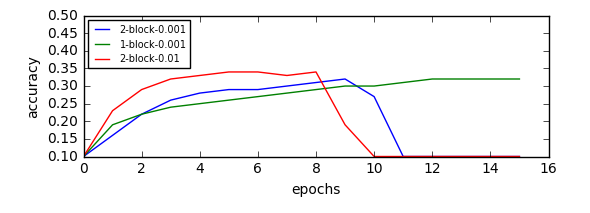
\includegraphics[scale=0.7]{wykres}
			\end{figure}
			        \paragraph{Discussion} 
			        
			        \begin{itemize}
			                \item Implementation which is using tf.nn.conv2d 2 times in each binarization process is much slower. 
			                \item Network with binarized both weights and activation is much harder to learn. In 2-layer Lenet the results were still very stable, but adding more layers, for example 14 in 2-blocks ResNet made network able to learn only during first few rounds of computation.
			                \item Smaller learning rate allows network to learn. Unfortunately the problem of deeper network still occurs, so the advantage of ResNet is not preserved.
			        \end{itemize}


\begin{thebibliography}{99}
\addcontentsline{toc}{chapter}{Bibliography}

\bibitem{understanding} Chiyuan Zhang, Samy Bengio, Moritz Hardt, Benjamin Recht, Oriol Vinyals, \textit{Understanding deep learning requires rethinking generalization}, https://arxiv.org/abs/1611.03530 (2016)

\bibitem{xornet} Mohammad Rastegari, Vicente Ordonez, Joseph Redmon, Ali Farhadi, \textit{XNOR-Net: ImageNet Classification Using Binary Convolutional Neural Networks}, https://arxiv.org/abs/1603.05279 (2016)

\bibitem{binaryConnect} Matthieu Courbariaux, Yoshua Bengio, Jean-Pierre David, \textit{BinaryConnect: Training Deep Neural Networks with binary weights during propagations}, https://arxiv.org/abs/1511.00363 (2015)

\bibitem{dorefa} Shuchang Zhou, Yuxin Wu, Zekun Ni, Xinyu Zhou, He Wen, Yuheng Zou, \textit{DoReFa-Net: Training Low Bitwidth Convolutional Neural Networks with Low Bitwidth Gradients}, https://arxiv.org/abs/1606.06160 (2016)

\bibitem{resnet} Kaiming He, Xiangyu Zhang, Shaoqing Ren, Jian Sun, \textit{Deep Residual Learning for Image Recognition}, https://arxiv.org/abs/1512.03385 (2015)

\end{thebibliography}


\end{document}
